\chapter{汽化器侧出口堵销}
\begin{figure}[htbp]
\centering
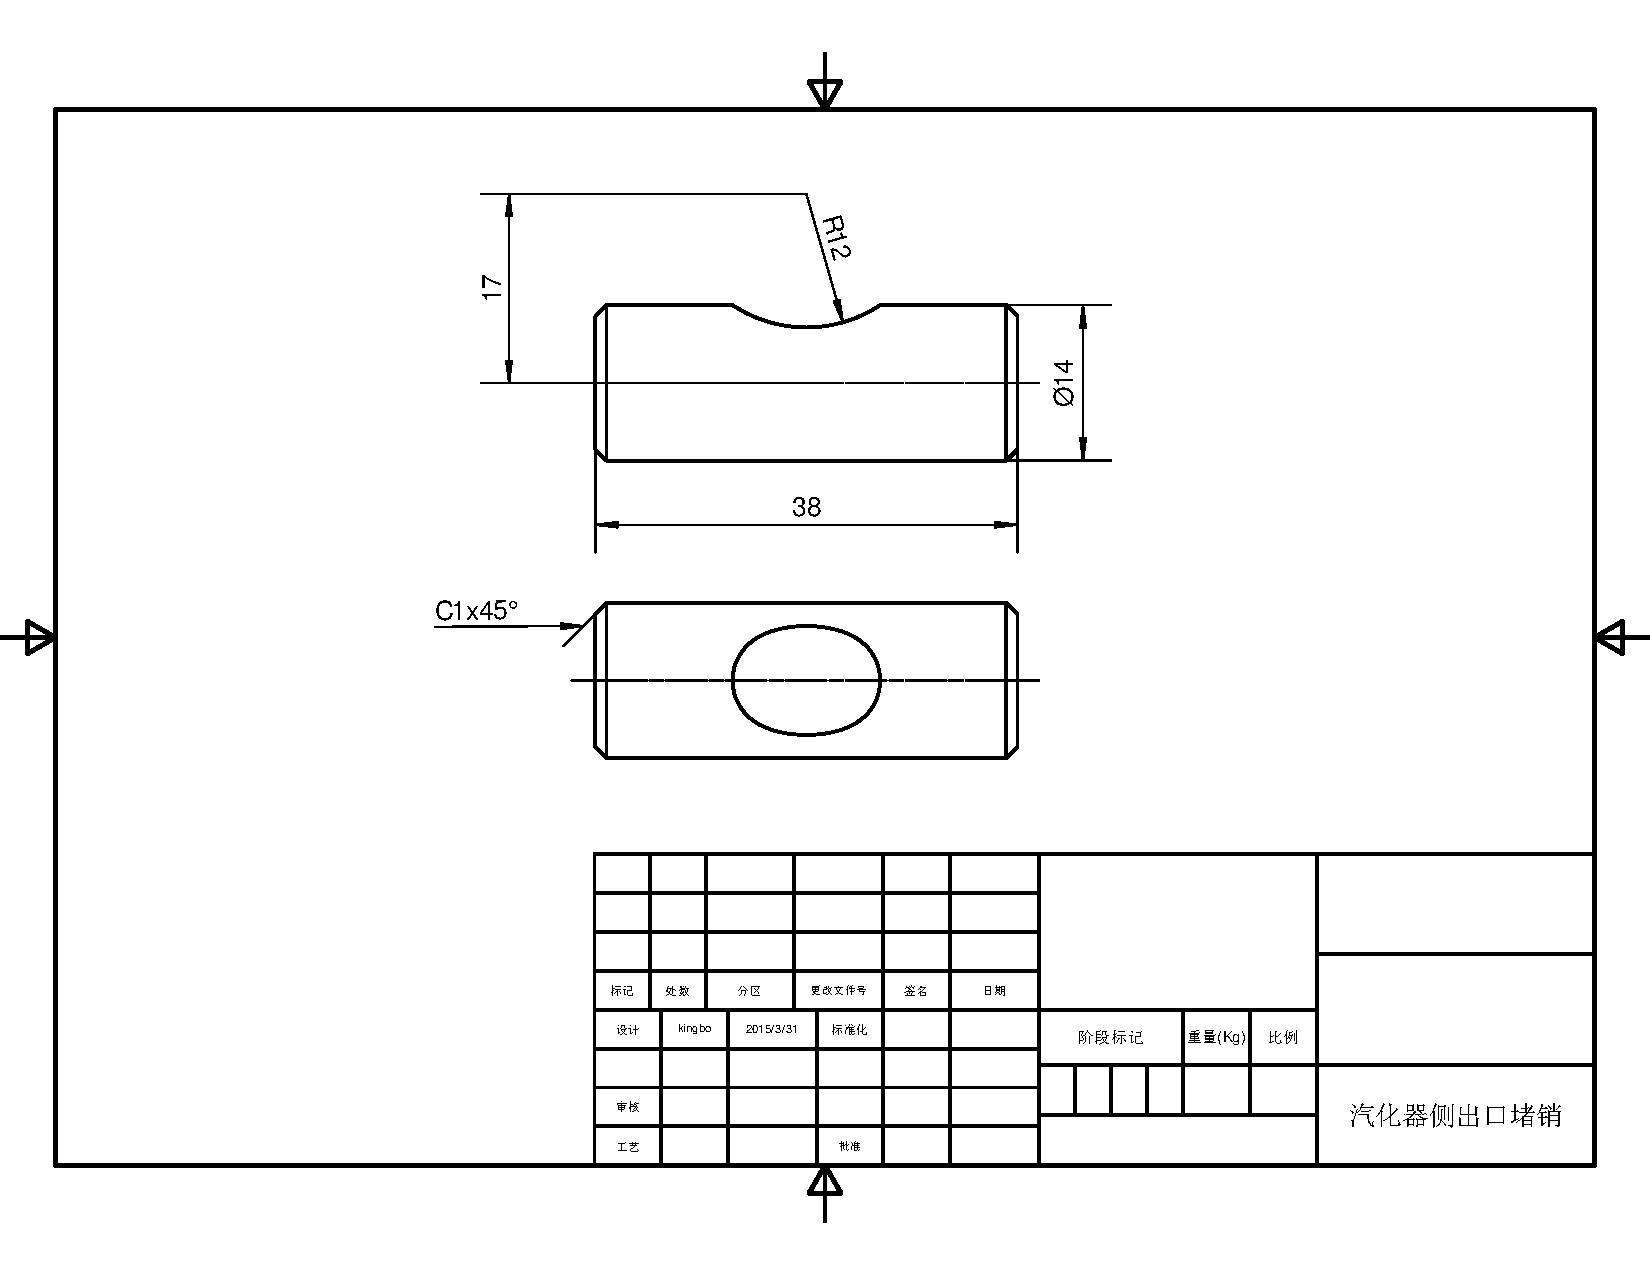
\includegraphics[scale=0.45,angle=-90]{chechukouxiao}
\caption{汽化器侧出口堵销零件图}\label{fig:chechukouxiao}
\end{figure}
%AutoCAD作为国际上广泛使用的流行的绘图工具,它具有较强的二维绘图和三维绘图功能,欢迎来到AutoCAD的三维世界,
本章我们的目标是用AutoCAD制作图\ref{fig:chechukouxiao}所示的航模发动机汽化器侧出口堵销零件的三维模型。本章将学习以下内容:
\begin{itemize}
	\item 截交体的概念
	\item 差集操作
\end{itemize}
\section{汽化器侧出口堵销建模}
\begin{procedure}
\item 切换视图方向

\begin{lstlisting}
命令: -view 
输入选项 [?/删除(D)/正交(O)/恢复(R)/保存(S)/设置(E)/窗口(W)]:left
\end{lstlisting}

\begin{lstlisting}
命令: -view 
输入选项 [?/删除(D)/正交(O)/恢复(R)/保存(S)/设置(E)/窗口(W)]:swiso 
\end{lstlisting}
\item 构建堵销基础圆柱体
\begin{lstlisting}
命令: cylinder
指定底面的中心点或 [三点(3P)/两点(2P)/切点、切点、半径(T)/椭圆(E)]:
指定底面半径或 [直径(D)]: 7
指定高度或 [两点(2P)/轴端点(A)]: 38
\end{lstlisting}

\item 构建切除圆柱体

\begin{lstlisting}
命令: -view 
输入选项 [?/删除(D)/正交(O)/恢复(R)/保存(S)/设置(E)/窗口(W)]:top
\end{lstlisting}

\begin{lstlisting}
命令: -view 
输入选项 [?/删除(D)/正交(O)/恢复(R)/保存(S)/设置(E)/窗口(W)]:swiso 
\end{lstlisting}

\begin{lstlisting}
命令: CYLINDER
指定底面的中心点或 [三点(3P)/两点(2P)/切点、切点、半径(T)/椭圆(E)]:
指定底面半径或 [直径(D)] <7.0000>: 12
指定高度或 [两点(2P)/轴端点(A)] <38.0000>: 14
\end{lstlisting}
\item 绘制辅助线
\begin{lstlisting}
命令: line
指定第一个点:
指定下一点或 [放弃(U)]: 
指定下一点或 [放弃(U)]:
\end{lstlisting}
\begin{lstlisting}
命令: line
指定第一个点:
指定下一点或 [放弃(U)]:
指定下一点或 [放弃(U)]:
\end{lstlisting}
\item 构建切口
\begin{lstlisting}
命令: offset
当前设置: 删除源=否  图层=源  OFFSETGAPTYPE=0
指定偏移距离或 [通过(T)/删除(E)/图层(L)] <通过>:  17
选择要偏移的对象,或 [退出(E)/放弃(U)] <退出>:
指定要偏移的那一侧上的点,或 [退出(E)/多个(M)/放弃(U)] <退出>:
选择要偏移的对象,或 [退出(E)/放弃(U)] <退出>:
\end{lstlisting}
\begin{lstlisting}
命令: move
选择对象: 找到 1 个
选择对象:
指定基点或 [位移(D)] <位移>:
指定第二个点或 <使用第一个点作为位移>:
\end{lstlisting}
\item 删除辅助线
\begin{lstlisting}
命令: erase
选择对象: 找到 1 个
选择对象: 找到 1 个,总计 2 个
选择对象: 找到 1 个,总计 3 个
选择对象:
\end{lstlisting}
\item 构建倒角边
\begin{lstlisting}
命令:  CHAMFEREDGE
距离 1 = 1.0000,距离 2 = 1.0000
选择一条边或 [环(L)/距离(D)]: d
指定距离 1 或 [表达式(E)] <1.0000>:
指定距离 2 或 [表达式(E)] <1.0000>:
选择一条边或 [环(L)/距离(D)]:
选择同一个面上的其他边或 [环(L)/距离(D)]:
选择同一个面上的其他边或 [环(L)/距离(D)]:
按 Enter 键接受倒角或 [距离(D)]:
\end{lstlisting}
\item 切换视觉样式
\begin{lstlisting}
命令: vscurrent
输入选项 [二维线框(2)/线框(W)/隐藏(H)/真实(R)/概念(C)/着色(S)/带边缘着色(E)/灰度(G)/勾画(SK)/X 射线(X)/其他(O)] <二维线框>: g
\end{lstlisting}

\item 保存模型
\end{procedure}
\endinput